\begin{figure*}[t]
\begin{subfigure}{0.3\textwidth}
   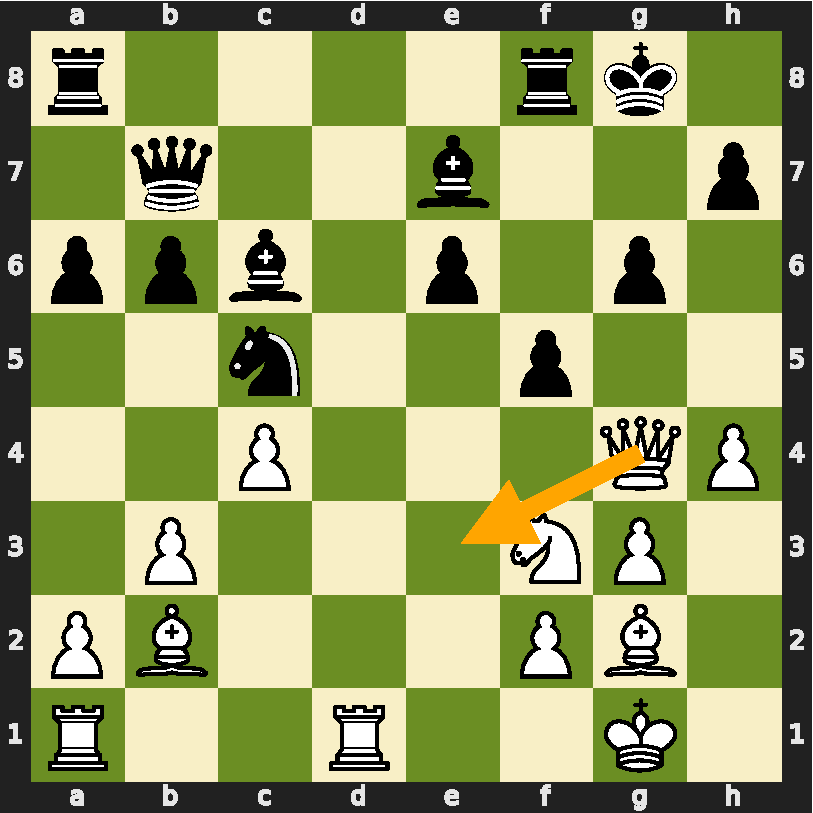
\includegraphics[width=\linewidth]{figures/board_syntax.pdf}
   \caption{\emph{Syntax}: Queen can move like all other piece types except for knight.} \label{fig:error_syntax}
\end{subfigure}
\hspace*{\fill}
\begin{subfigure}{0.3\textwidth}
   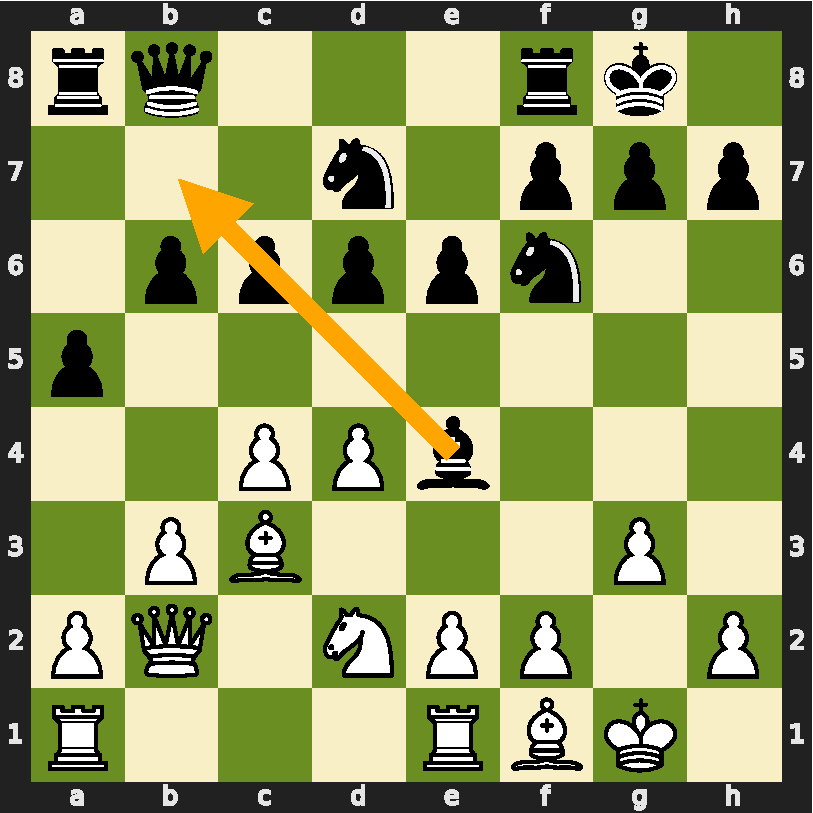
\includegraphics[width=\linewidth]{figures/board_path.pdf}
   \caption{\emph{Path Obstruction}: The pawn at \pos{c6} is blocking the bishop.} \label{fig:error_path}
\end{subfigure}
\hspace*{\fill}
\begin{subfigure}{0.3\textwidth}
   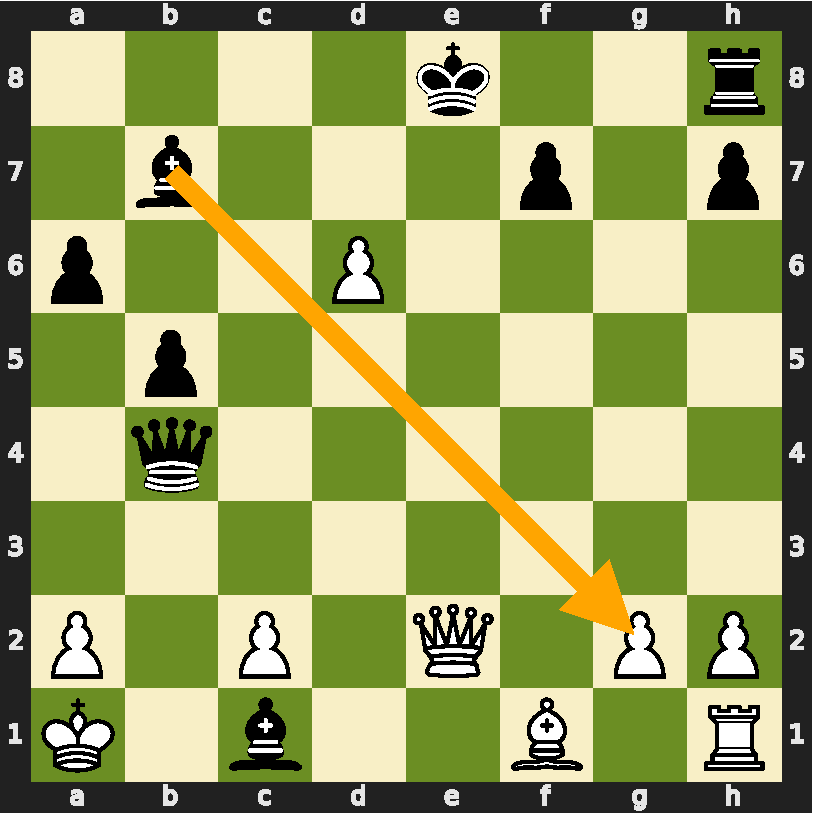
\includegraphics[width=\linewidth]{figures/board_pseudo.pdf}
   \caption{\emph{Pseudo Legal}: The black king remains in check.} \label{fig:error_pseudo}
\end{subfigure}
\caption{Instances of the three prominent categories of illegal ending square predictions.}
\label{fig:error_categories}
\end{figure*}


\begin{table*}[ht]
	\centering{
		\caption{Error counts for ending square prediction.}
		\label{tab:error_analysis}
\begin{tabular}{llcccccc}
	\toprule
	& \multirow{2.5}{*}{Model}   &  \multicolumn{3}{c}{Actual}      &   \multicolumn{3}{c}{Other}    \\
	\cmidrule(lr){3-5}\cmidrule(lr){6-8}
	&        & Syntax & Path Obst. & Pseudo Leg.  & Syntax & Path Obst. & Pseudo Leg.\\
	
	\midrule
	
	\multirow{4}{*}{Train-S} 
	& UCI 				& 168 & 48 & 40 & 173 & \phantom{1}90 & \phantom{1}80 \\ 
	& UCI + RAP			& \phantom{1}20 & 58 & 38 & \phantom{1}17 & \phantom{1}96 & \phantom{1}81\\
	& UCI + \piecetype	& \phantom{11}1 & 99 & 29 & \phantom{11}3 & 126 & \phantom{1}81\\
	& Performer 		& 235 			& 56 & 53 & 243 & \phantom{1}70 & 106\\
	
	\midrule
	
	\multirow{4}{*}{Train-M} 
	& UCI 				& \phantom{1}16 & 30 & 25 & \phantom{1}15 & \phantom{1}54 & \phantom{1}72 \\ 
	& UCI + RAP			& \phantom{11}3 & 30 & 18 & \phantom{11}7 & \phantom{1}56 & \phantom{1}55\\
	& UCI + \piecetype	& \phantom{11}0 & 36 & 17 & \phantom{11}3 & \phantom{1}59 & \phantom{1}53 \\
	& Performer			& \phantom{1}41 & 27 & 40 			& \phantom{1}42 	& \phantom{1}45 & 108\\

	\midrule
	
	\multirow{4}{*}{Train-L} 
	&  UCI 				& \phantom{11}1 & 10 & 12 & \phantom{11}4 & \phantom{1}26 & \phantom{1}49 \\ 
	& UCI + RAP			& \phantom{11}0 & 19 & 11 & \phantom{11}3 & \phantom{1}29 & \phantom{1}36 \\
	& UCI + \piecetype 	& \phantom{11}0 & 13 & \phantom{1}5 & \phantom{11}3 & \phantom{1}13 & \phantom{1}31\\
	& Performer			& \phantom{11}8 & 18 & 16 & \phantom{11}9 & \phantom{1}23 & \phantom{1}63 \\
	\bottomrule
\end{tabular}
	}
\end{table*}


\section{Error Analysis}
\label{sec:error_analysis}

In this section we analyze errors %
on the ending square prediction task. 
Incorrect predictions for this task %
can be (exhaustively) categorized into four categories:

\begin{itemizesquish}
	\itemsep0em 
	\item {\em Unreachable}: The predicted ending square cannot be reached %
	by any possible piece type %
	at the starting square regardless of the board state. 
	\item {\em Syntax}: The predicted ending square cannot be reached %
	by the piece type present at the starting square regardless of the board state. This error indicates failure at tracking the piece type present at the starting square. 
	\item {\em Path Obstruction}: The predicted ending square cannot be reached 
	because there are other pieces obstructing the %
	path. This error indicates failure at tracking other pieces on the board or a lack of %
	understanding that for all piece types except the knight, the path %
	must be clear. %
	For example, in Figure~\ref{fig:error_path}, the pawn at \pos{c6} blocks the bishop's move from \pos{e4} to \pos{b7}.
	\item {\em Pseudo Legal}: 
	The move is illegal because the moving player's king is in check at the end of the move. 
\end{itemizesquish}
Table~\ref{tab:error_analysis} shows error counts for the ending square prediction task. 
For brevity we omit unreachable errors since they are rare ($< 5$ for all models).


Errors across all categories decrease with more training data. For syntax errors this reduction is particularly dramatic, decreasing by roughly an order of magnitude when moving from Train-S to Train-M. %
In contrast, both path obstruction and pseudo legal errors decline more gradually.
Determining whether a path is blocked or if the king is in check requires a computation involving multiple piece locations which all need to be computed from the move  history. 
These trends suggest that identifying the piece type at a starting square 
requires data but is learnable, while keeping track of all \emph{other} pieces  on the board remains challenging even with large training sets.

UCI + RAP %
consistently outperforms %
UCI in syntax errors, %
the differences being largest for the small training sets. This validates our hypothesis that RAP can aid the model in piece tracking (Section~\ref{sec:rap_board}). Across other error categories we don't see consistent trends, suggesting piece tracking improvements do not necessarily translate to other error categories. The Performer generally makes more errors than the transformers, especially in the syntax category. The partial attention in the Performer may be limiting its ability to attend to the most relevant prior positions to determine the piece type at the given starting square. 

Predicting ending squares for the actual move made (``Actual'') is easier than for a randomly chosen legal move (``Other''). However, the syntax errors are comparable between the two settings, while there are many more path obstruction and pseudo legal errors for the Other instances. 
	The higher error rate for these categories could be because:
	\begin{itemizesquish}
		\item Avoiding path obstruction and check are difficult functions to learn and may therefore be being ``mimicked'' from training data rather than being learned as a general algorithmic function.
		\item The model is trained on only actual games with emphasis on meaningful moves rather than legal moves. We observe that some of the Other instances lack any ``meaningful" continuations (Appendix~\ref{sec:app_error_analysis}).
		\item There's a distribution shift between piece types moved in actual moves vs randomly chosen legal moves. 
		For example, the End-Actual task has only about 13\% prompts for moves made by king in comparison to the 33\% for the End-Other task (Appendix~\ref{sec:data_stats}).  We find that moves made by king have a higher chance of resulting in pseudo legal errors in comparison to other piece types (Appendix~\ref{sec:pseudo_legal}).  
	\end{itemizesquish} 







\subsection{Detailed Error Analysis}
\label{sec:app_error_analysis}
\begin{figure*}[!ht]
	\centering{
		\hspace*{\fill}
\begin{subfigure}{0.43\textwidth}
   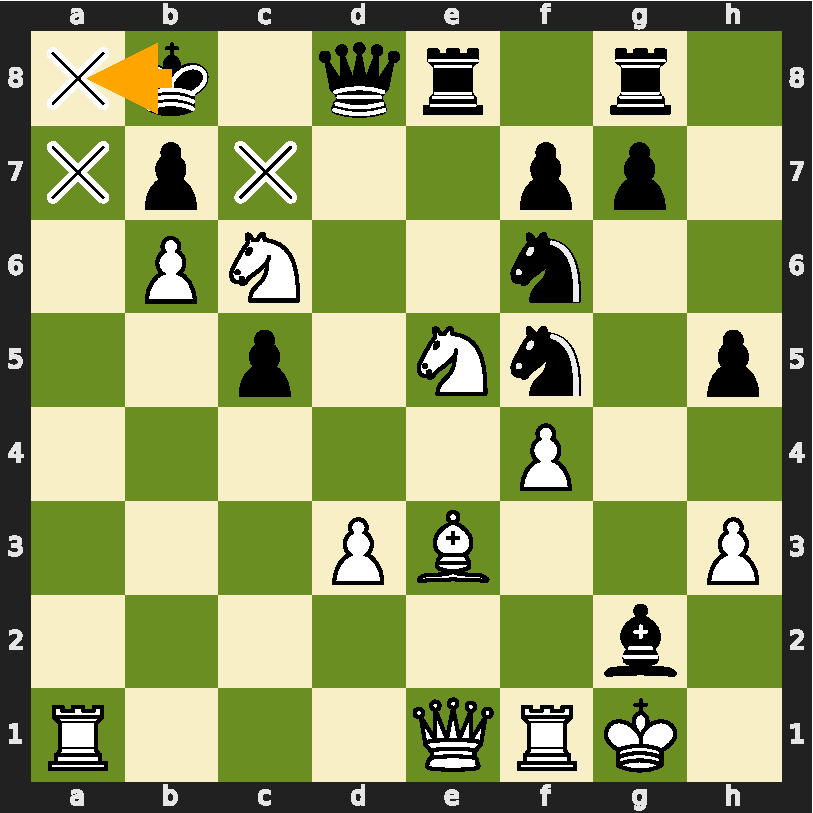
\includegraphics[width=\linewidth]{figures/board_check_king.pdf}
   \caption{\emph{Check + King}: Black king is in check and the predicted ending square is already covered by the white rook on \pos{a1}.} 
   \label{fig:error_check_king}
\end{subfigure}
\hspace*{\fill}
\begin{subfigure}{0.43\textwidth}
	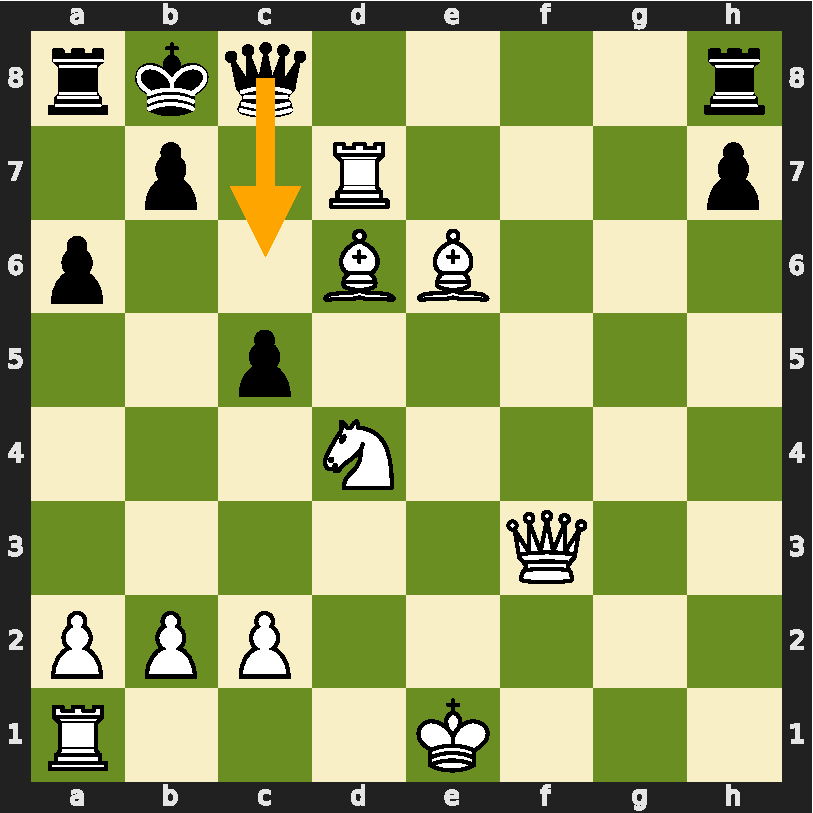
\includegraphics[width=\linewidth]{figures/board_check_no_king.pdf}
	\caption{\emph{Check + Other}: Black king is in check and the only legal move for the black queen is \pos{c7} but the model predicts \pos{c6}.} 
	\label{fig:error_check_no_king}
\end{subfigure}
\hspace*{\fill}
\\[1em]
\hspace*{\fill}
\begin{subfigure}{0.43\textwidth}
   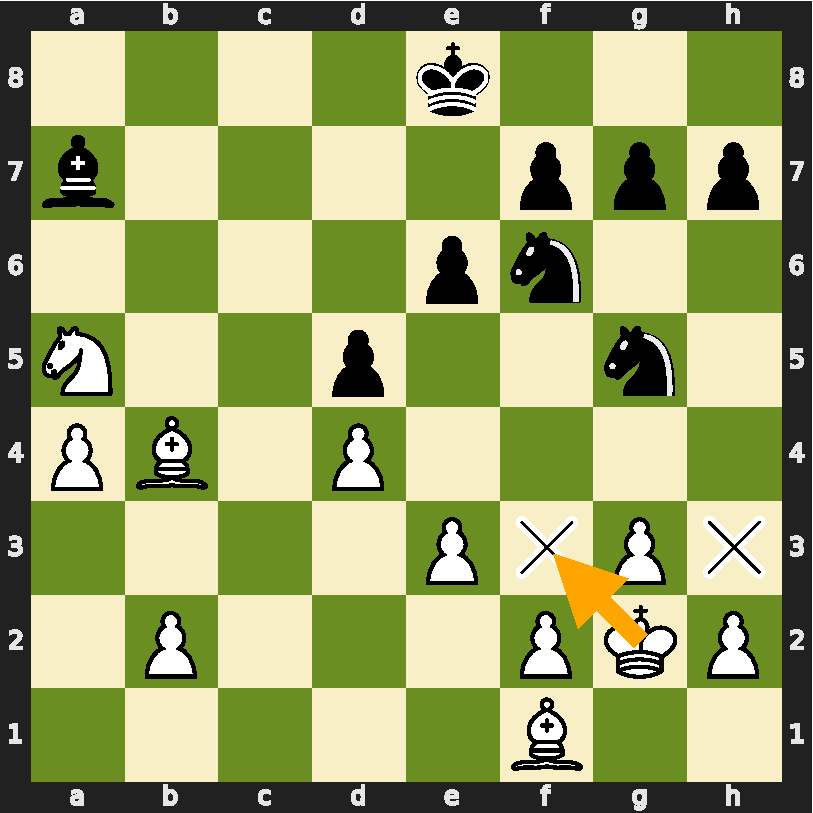
\includegraphics[width=\linewidth]{figures/board_no_check_king.pdf}
   \caption{\emph{No Check + King}: The predicted ending square \pos{f3} for the white king is guarded by the black knight at \pos{g5}.} 
   \label{fig:error_no_check_king}
\end{subfigure}
\hspace*{\fill}
\begin{subfigure}{0.43\textwidth}
	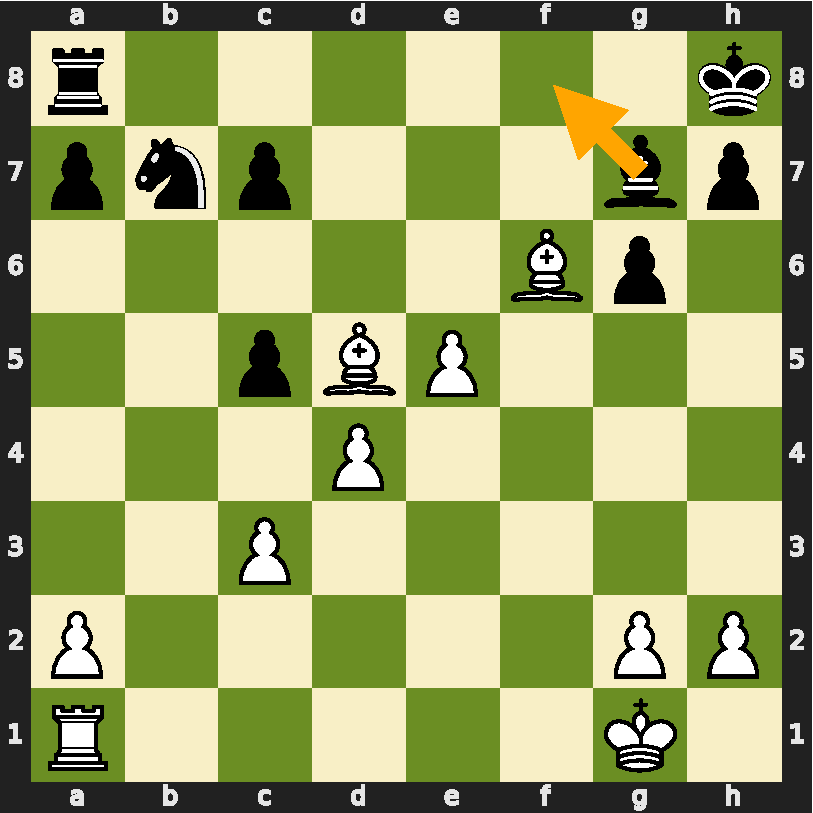
\includegraphics[width=\linewidth]{figures/board_no_check_no_king.pdf}
	\caption{\emph{No Check + Other}: The predicted ending square \pos{f8} for the black bishop exposes its king to the white bishop at \pos{f6}. } 
	\label{fig:error_no_check_no_king}
\end{subfigure}
\hspace*{\fill}
\caption{Four combinations of the king being in check or not, and if the king is moved or not, that can result in Pseudo Legal errors.}
\label{fig:pseudo_legal_errors}
}
\end{figure*}





In this section we conduct a more in-depth analysis of errors made by the UCI model trained with Train-L for the ending square prediction task. We limit our focus to the two main error categories, namely, Pseudo Legal and Path Obstruction.



\begin{table}[t]
	\centering{
		\caption{Pseudo Legal error counts for different categories. For the total column we remove instances with errors of other category.}
		\label{tab:pseudo_legal}
		\begin{tabular}{lcccc}
			\toprule
			Category & \multicolumn{2}{c}{End-Actual} & \multicolumn{2}{c}{End-Other}\\
			& Errors & Total & Errors & Total \\
			\midrule
			Check + King 		& 1	& \phantom{1}27  & \phantom{1}2 & \phantom{1}20	\\
			Check + Other 		& 7	& \phantom{1}26  & 16			& \phantom{1}33 \\ 			 
			No Check + King 	& 4	& 101 			& 31 			& 296	\\ 
			No Check + Other 	& 0 & 835 &	\phantom{1}0  			& 619	\\ 
			\midrule
			Total 				& 12 & 989  	& 49 			& 968\\\bottomrule
		\end{tabular}
	}
	
\end{table}

\begin{table}[ht]
	\caption{Piece type counts for Path Obstruction error category. For the total column we remove instances with errors of other category.}
	\label{tab:path_obs}
	\centering
	\begin{tabular}{lcccc}
		\toprule
		Piece type & \multicolumn{2}{c}{End-Actual} & \multicolumn{2}{c}{End-Other} \\ %
		& Errors & Total & Errors & Total \\
		\midrule
		Rook (\pos{R}) 	& 	3 	& 355	& 17  			& 267    		\\ 
		Knight (\pos{N}) 	& 	1  	& 144	& \phantom{1}1 	& 131 			\\  
		Bishop (\pos{B}) 	& 	1 	& 162	& \phantom{1}3 	& 164 			\\
		Queen (\pos{Q}) 	& 	4  	& 202	& \phantom{1}4  & \phantom{1}99	\\ 
		King (\pos{K}) 	& 	1  	& 124 	& \phantom{1}1  & 284			\\
		\midrule
		Total 		& 	10 	& 987  	& 26 			& 945\\\bottomrule
	\end{tabular}
\end{table}

\subsection{Pseudo Legal Errors}
\label{sec:pseudo_legal}
We conduct our analysis by categorizing instances according to: (a) if the king was in check before the current move, and (b) if the king is being moved in the current move. 
Figure~\ref{fig:pseudo_legal_errors} presents one instance for each of these four categories.
Table~\ref{tab:pseudo_legal} presents the breakdown of errors for the End-Actual and End-Other instances. The key takeaways from the error categorization are: (a) Error counts for ``Check + King" and ``No Check + Other" are relatively low and similar across the two classes of prompts. (b) ``Check + Other" i.e.\ the king is in check and some other piece is moved, has high count for both the splits. The particularly high count for End-Other could be explained by the lack of ``meaningful" moves for certain prompts of this kind. For example, in figure~\ref{fig:error_check_no_king} the prompt asks for the queen at \pos{c8} to move, and the only legal continuation is for the queen to bring itself to the firing line at \pos{c7}. (c) ``No Check + King"  is another common error category. 
The significantly higher error count for End-Other could be due to a combination of the higher frequency of such prompts and the out-of-distribution prompts.
 


\begin{figure*}[!ht]
	\centering{
		\hspace*{\fill}
		\begin{subfigure}{0.4\textwidth}
			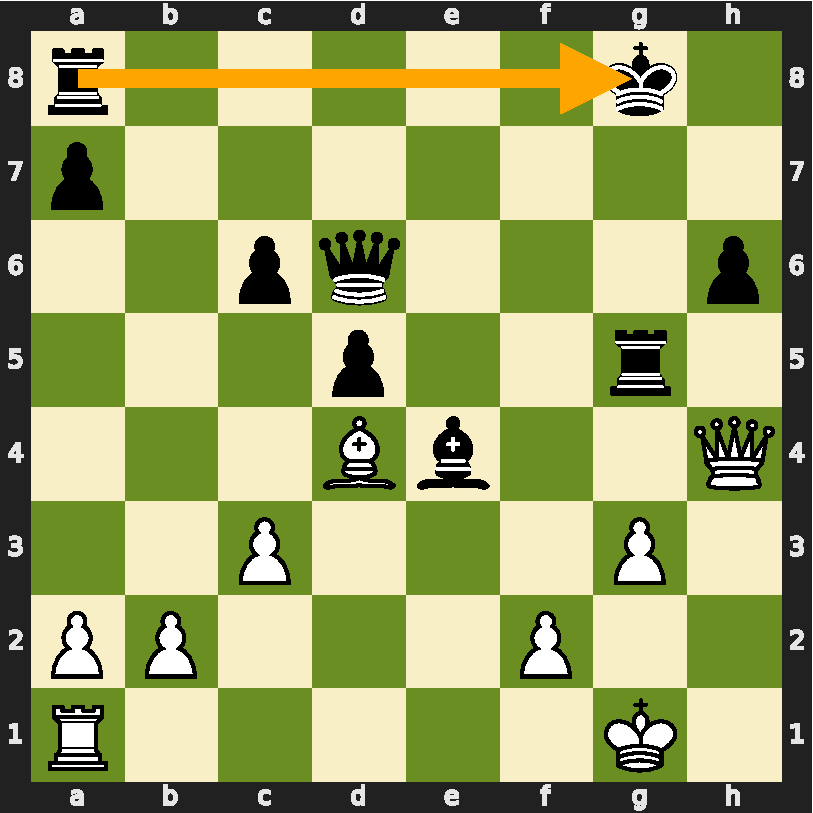
\includegraphics[width=\linewidth]{figures/board_path_rook.pdf}
			\caption{Rook forgets about its own king at \pos{g8}!} 
			\label{fig:rook_path}
		\end{subfigure}
		\hspace*{\fill}
		\begin{subfigure}{0.4\textwidth}
			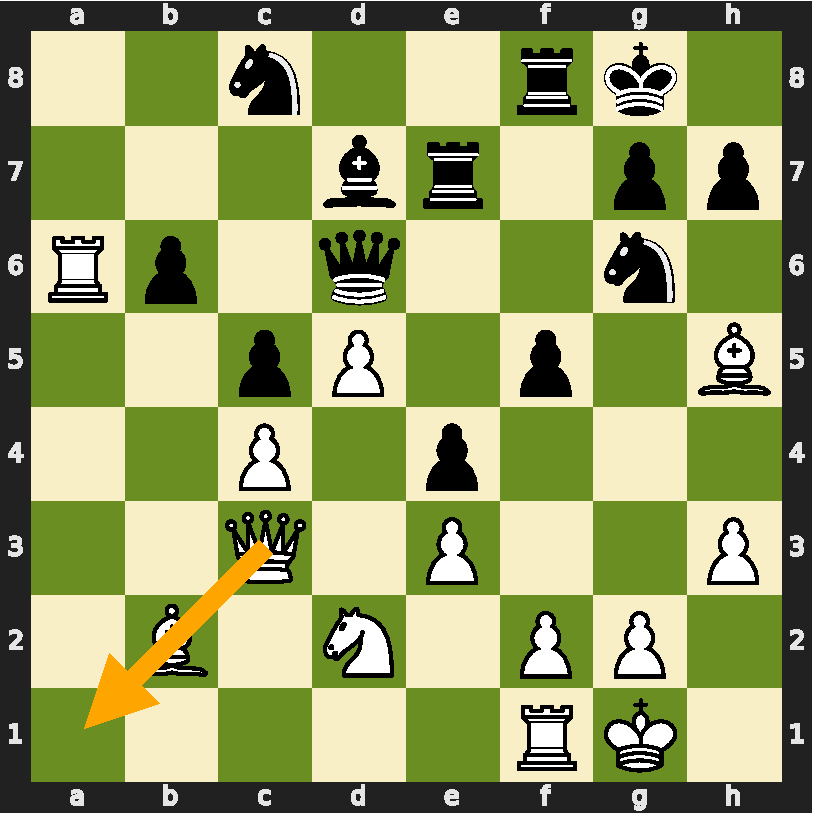
\includegraphics[width=\linewidth]{figures/board_path_queen.pdf}
			\caption{Bishop at \pos{b2} stands in the way of the queen.} 
			\label{fig:queen_path}
		\end{subfigure}
		\hspace*{\fill}
		\\[1em]
		\hspace*{\fill}
		\begin{subfigure}{0.4\textwidth}
			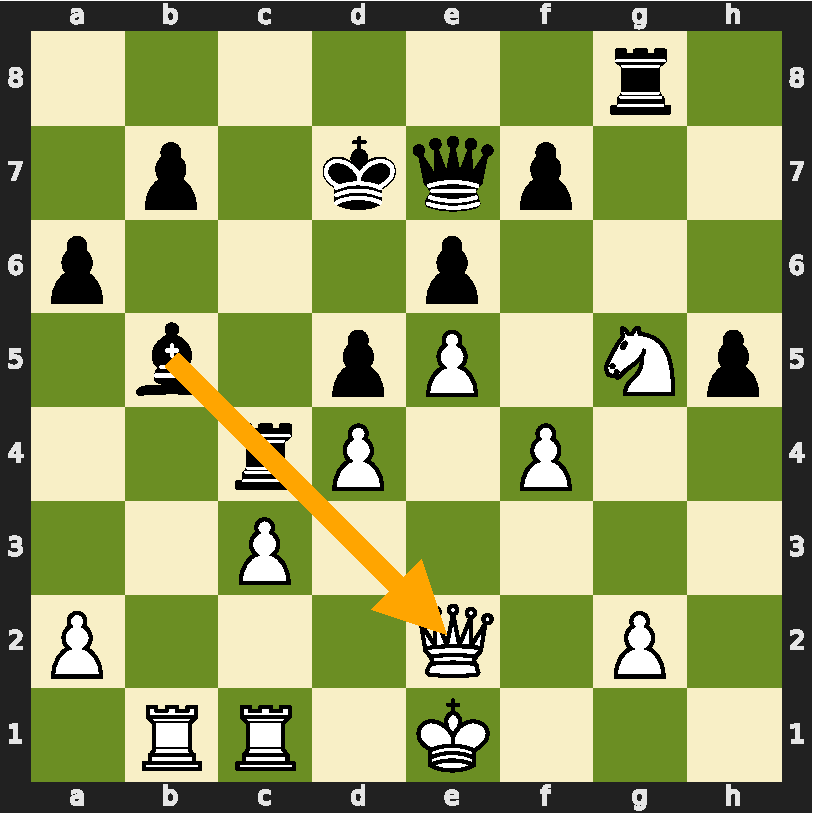
\includegraphics[width=\linewidth]{figures/board_path_bishop.pdf}
			\caption{Bishop forgets reality in pursuit of fantasy queen kill!} 
			\label{fig:bishop_path}
		\end{subfigure}
		\hspace*{\fill}
		\begin{subfigure}{0.4\textwidth}
			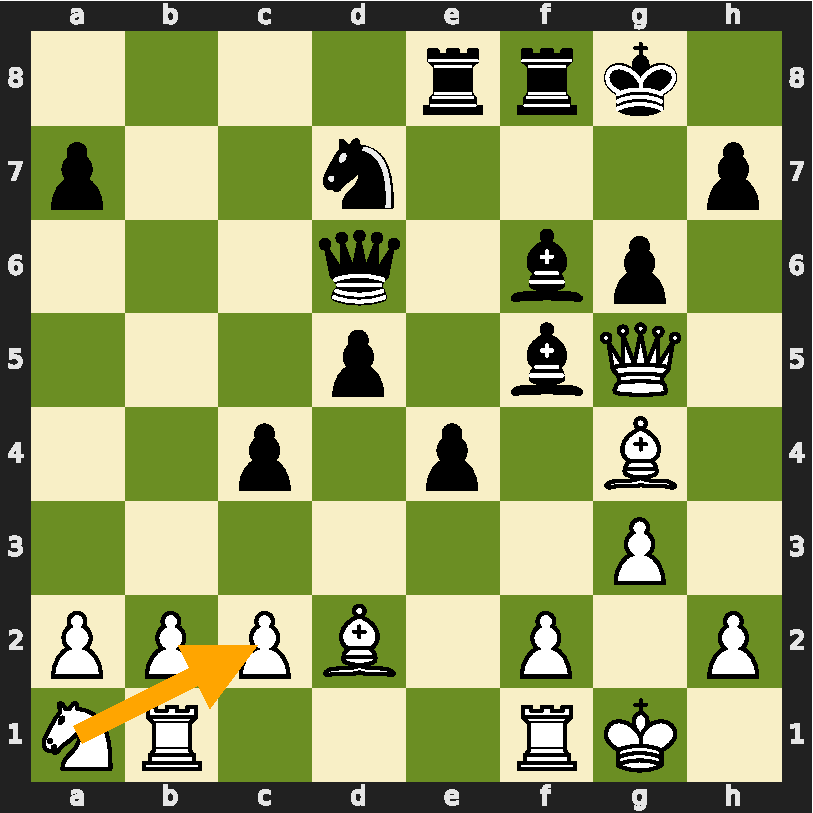
\includegraphics[width=\linewidth]{figures/board_path_knight.pdf}
			\caption{A trapped, frustrated knight is out to kill its own pawn!} 
			\label{fig:knight_path}
		\end{subfigure}
		\hspace*{\fill}
		\caption{Instances of Path Obstruction errors with different piece types.}
		\label{fig:path_obstruction}
	}
\end{figure*}


\begin{figure*}[!ht]
	\centering{
		\hspace*{\fill}
		\begin{subfigure}{0.35\textwidth}
			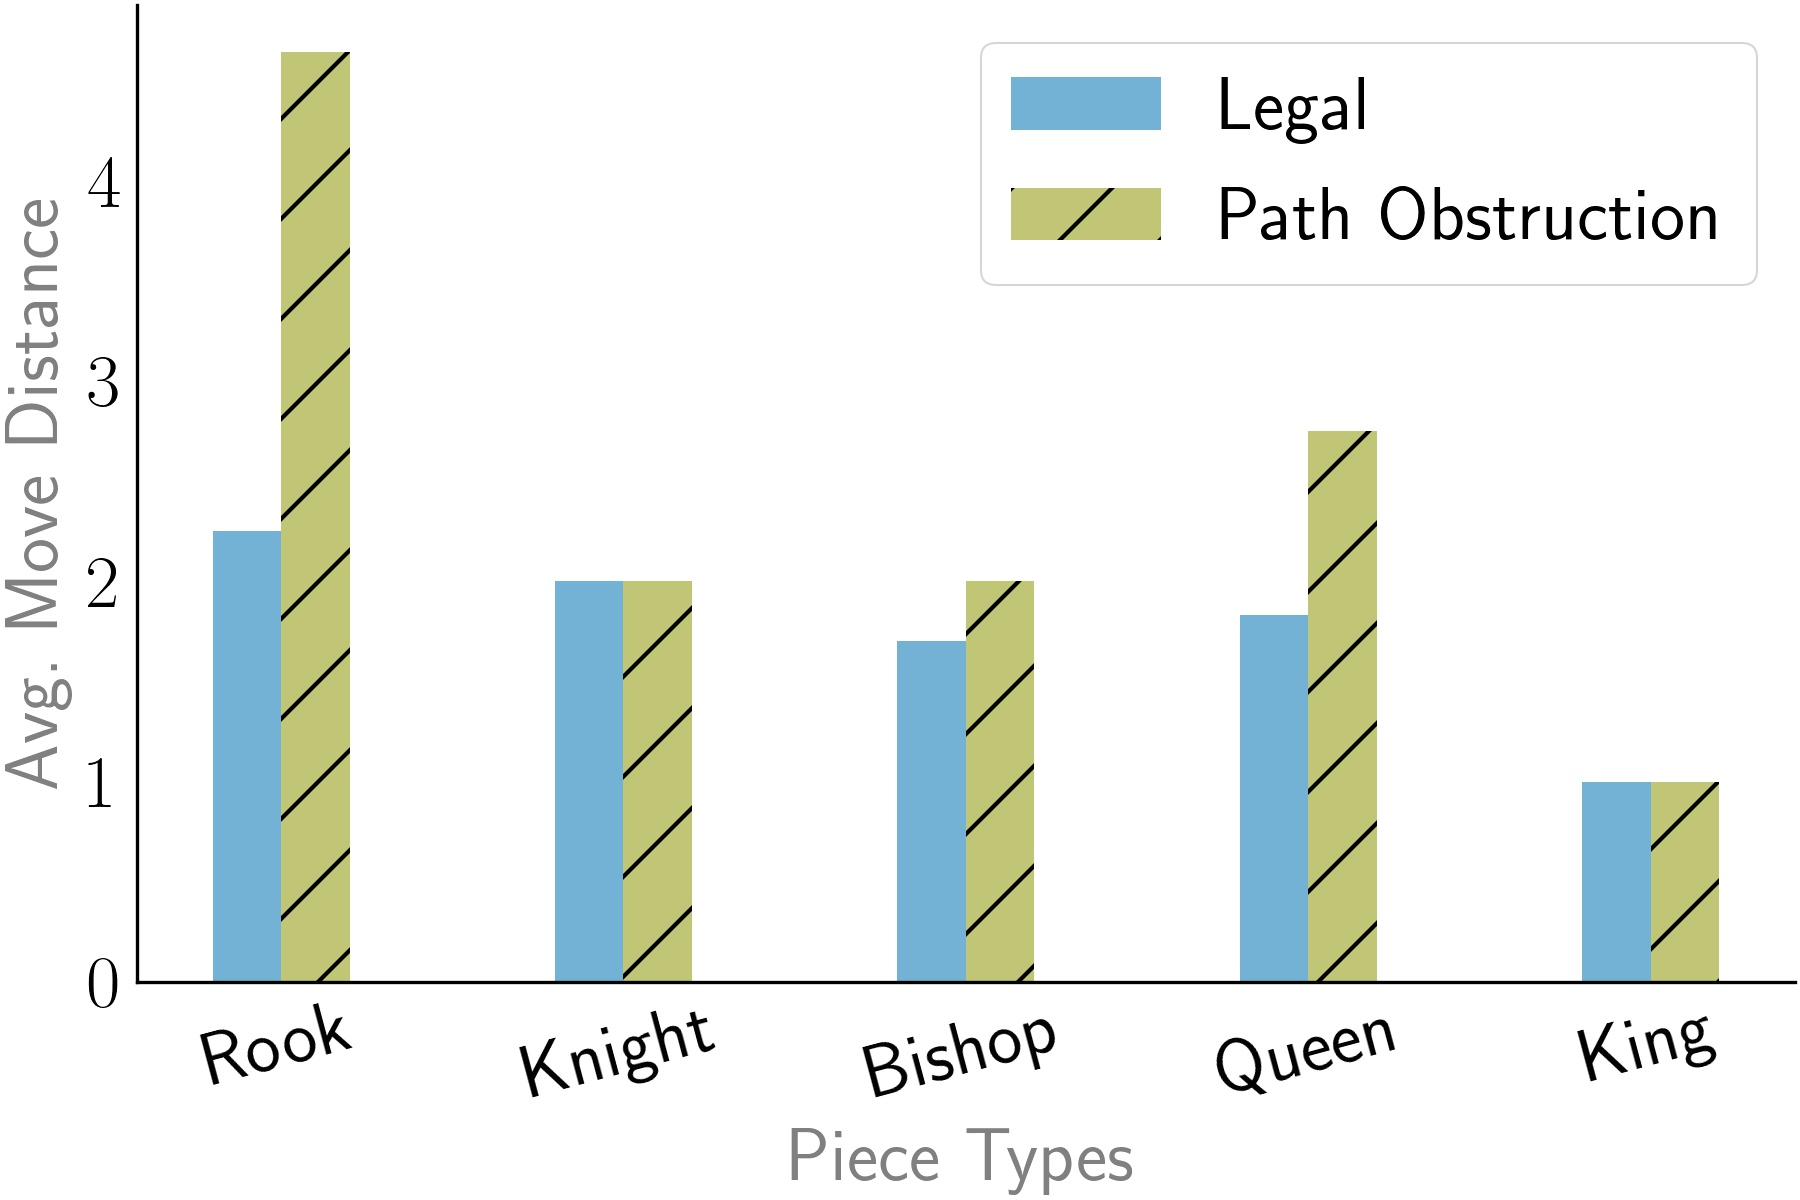
\includegraphics[width=\linewidth]{figures/path_obs_actual.jpg}
			\caption{End-Actual} 
			\label{fig:path_length_actual}
		\end{subfigure}
		\hspace*{\fill}
		\begin{subfigure}{0.35\textwidth}
			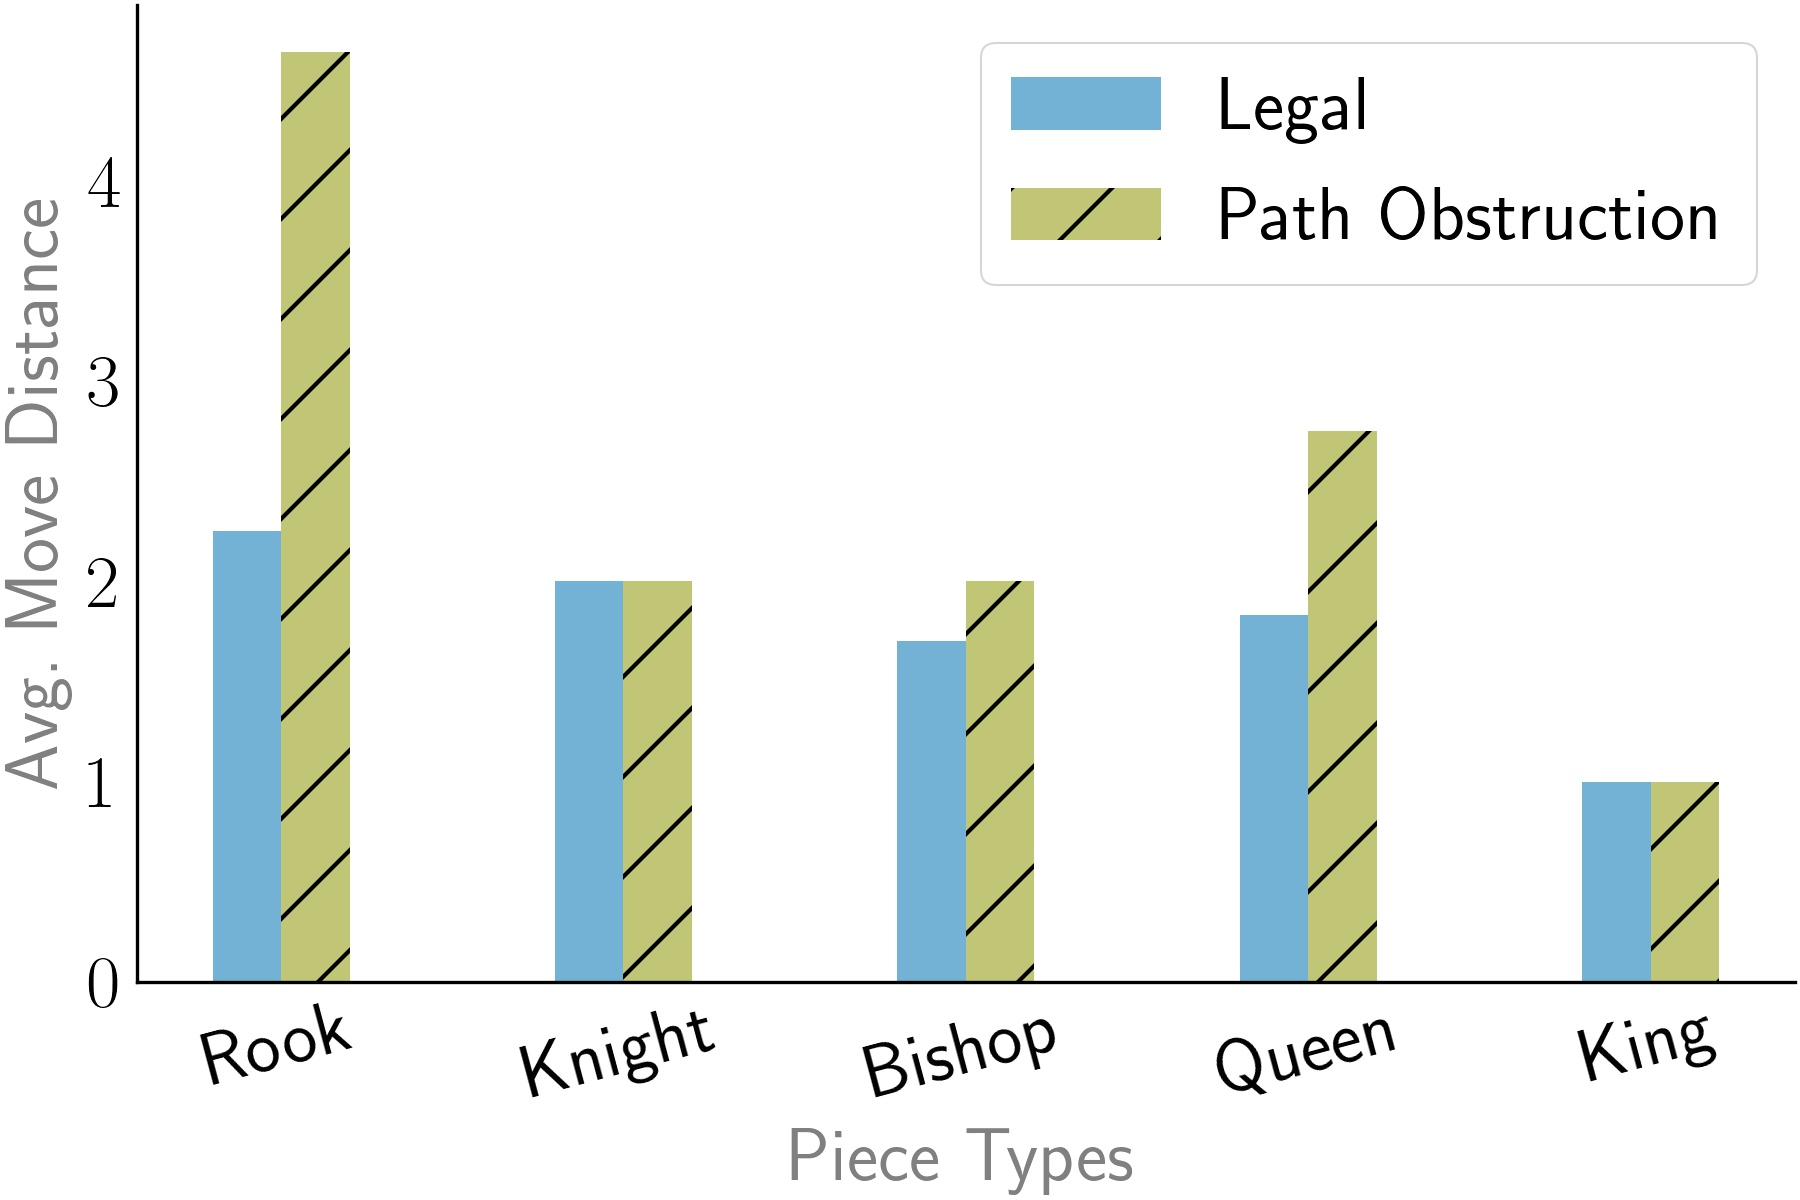
\includegraphics[width=\linewidth]{figures/path_obs_other.jpg}\\
			\caption{End-Other} 
			\label{fig:path_length_other}
		\end{subfigure}
	\hspace*{\fill}
\caption{Comparison of average path length of predicted moves for different piece types when the move is legal vs ones with path obstruction error.}
\label{fig:path_length}
}
\end{figure*}

\subsection{Path Obstruction}
Table~\ref{tab:path_obs} presents the path obstruction errors for different piece types for the End-Actual and End-Other task. Figure~\ref{fig:path_obstruction} represents instances of path obstruction error for different piece types.  
The error counts show that piece types with more dynamic movement except knight i.e. rook, bishop, and queen, have more path obstruction errors  (a knight just needs to avoid landing on its own piece to avoid path obstruction errors). 
These piece types also show a significant increase in frequency of path obstruction errors for End-Other in comparison to End-Actual. As in pseudo legal errors, this could again be due to the out-of-distribution nature of these prompts. Figure~\ref{fig:path_length} shows that the average path length for predicted moves with path obstruction error is significantly higher than the legal predictions for both the kinds of prompts (knight and king have a constant path length). \footnote{Path length is measured in number of king moves i.e. number of moves it will take a king to go from starting to ending square.}
